\section{گام پنجم: آزادسازی لایه‌ها \lr{(Fine-Tuning)} و کسب نمره اضافه}

با توجه به نتایج اولیه و به منظور بهبود چشمگیر دقت و کسب نمره‌ی اضافه \lr{(Extra Credit)}، یک آزمایش پیشرفته‌تر طراحی گردید. در مدل قبلی، تمامی لایه‌های استخراج ویژگی \lr{ResNet18} فریز شده بودند که برای درک ویژگی‌های ظریف چهره (میکرو-اکسپرشن‌ها) کافی نبود. بنابراین، تصمیم گرفته شد تا آخرین بلوک رزیدوال شبکه \lr{(layer4)} از حالت فریز خارج شده و فرآیند آموزش به مدت ۳۰ دوره \lr{(Epoch)} انجام پذیرد.

\subsection{تحلیل روند آموزش ۳۰ دوره‌ای و پدیده‌ی بیش‌برازش}
فرآیند آموزش حدود ۶۳ دقیقه به طول انجامید (میانگین ۱۲۵ ثانیه برای هر دوره). نمودارهای این فرآیند در ادامه آورده شده است.

\begin{figure}[h!]
    \centering
    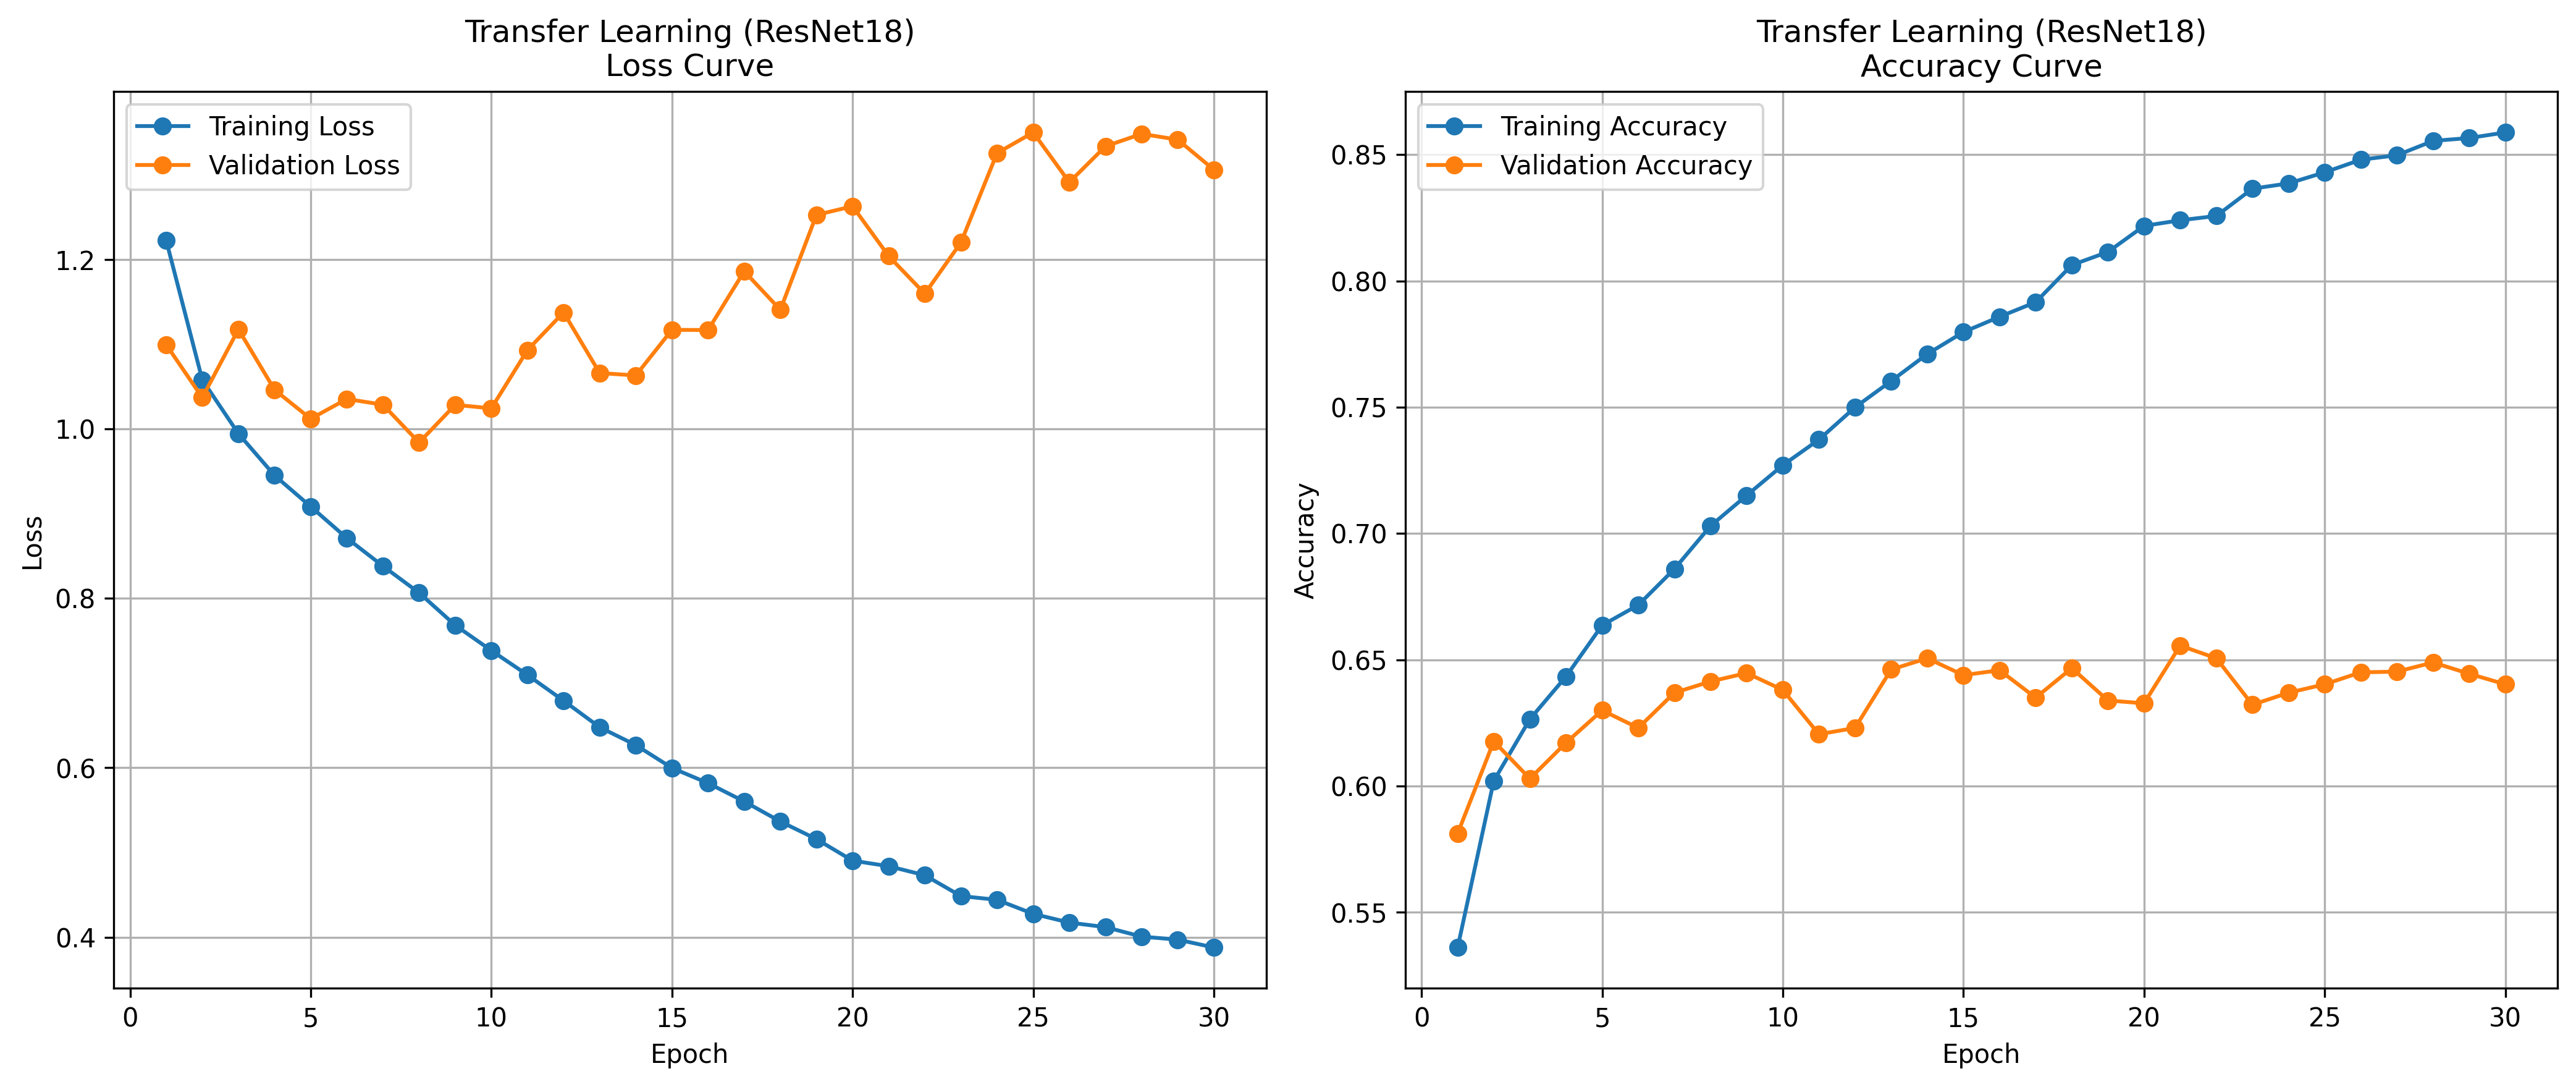
\includegraphics[width=1\textwidth]{images/tl_training_curves.png}
    \caption{منحنی‌های آموزش و اعتبارسنجی مدل \lr{Fine-Tuned ResNet18} طی ۳۰ دوره}
    \label{fig:finetune_curves}
\end{figure}

همان‌طور که در نمودار خطا \lr{(Loss Curve)} در شکل \ref{fig:finetune_curves} مشخص است، خطای آموزش تا پایان دوره سی‌ام به طور مداوم کاهش یافته و دقت آن به \lr{85.88\%} رسیده است. با این حال، خطای اعتبارسنجی از حدود دوره‌ی دهم شروع به افزایش ملایم می‌کند که نشانه‌ی واضحی از آغاز پدیده‌ی بیش‌برازش \lr{(Overfitting)} است. 

\begin{tipbox}[جلوگیری از افت عملکرد]
به لطف پیاده‌سازی سیستم ذخیره‌ی هوشمند \lr{(Model Checkpointing)}، مدل نهایی دچار این بیش‌برازش نشد؛ زیرا بهترین وزن‌های شبکه بر اساس بالاترین دقت اعتبارسنجی (دقت \lr{65.56\%} در دوره‌ی ۲۱) ذخیره و برای ارزیابی نهایی استفاده شدند.
\end{tipbox}

\newpage
\subsection{ارزیابی نهایی روی مجموعه‌ی آزمون \lr{(Test Set)}}
پس از بارگذاری بهترین وزن‌ها، مدل روی مجموعه‌ی آزمون ارزیابی شد و به دقت شگفت‌انگیز \lr{66\%} دست یافت. نتایج تفکیک‌شده به شرح زیر است:

\begin{itemize}
    \item \textbf{خشم \lr{(Angry)}:} \lr{F1-score: 0.56} | \lr{Recall: 0.54}
    \item \textbf{انزجار \lr{(Disgust)}:} \lr{F1-score: 0.60} | \lr{Recall: 0.69}
    \item \textbf{ترس \lr{(Fear)}:} \lr{F1-score: 0.48} | \lr{Recall: 0.40}
    \item \textbf{شادی \lr{(Happy)}:} \lr{F1-score: 0.86} | \lr{Recall: 0.89}
    \item \textbf{غم \lr{(Sad)}:} \lr{F1-score: 0.53} | \lr{Recall: 0.56}
    \item \textbf{تعجب \lr{(Surprise)}:} \lr{F1-score: 0.77} | \lr{Recall: 0.81}
    \item \textbf{خنثی \lr{(Neutral)}:} \lr{F1-score: 0.65} | \lr{Recall: 0.66}
\end{itemize}

\subsection{تحلیل ماتریس درهم‌ریختگی نهایی}
ماتریس درهم‌ریختگی این مدل ارتقایافته رسم گردید (شکل \ref{fig:cm2}).

\begin{figure}[h!]
    \centering
    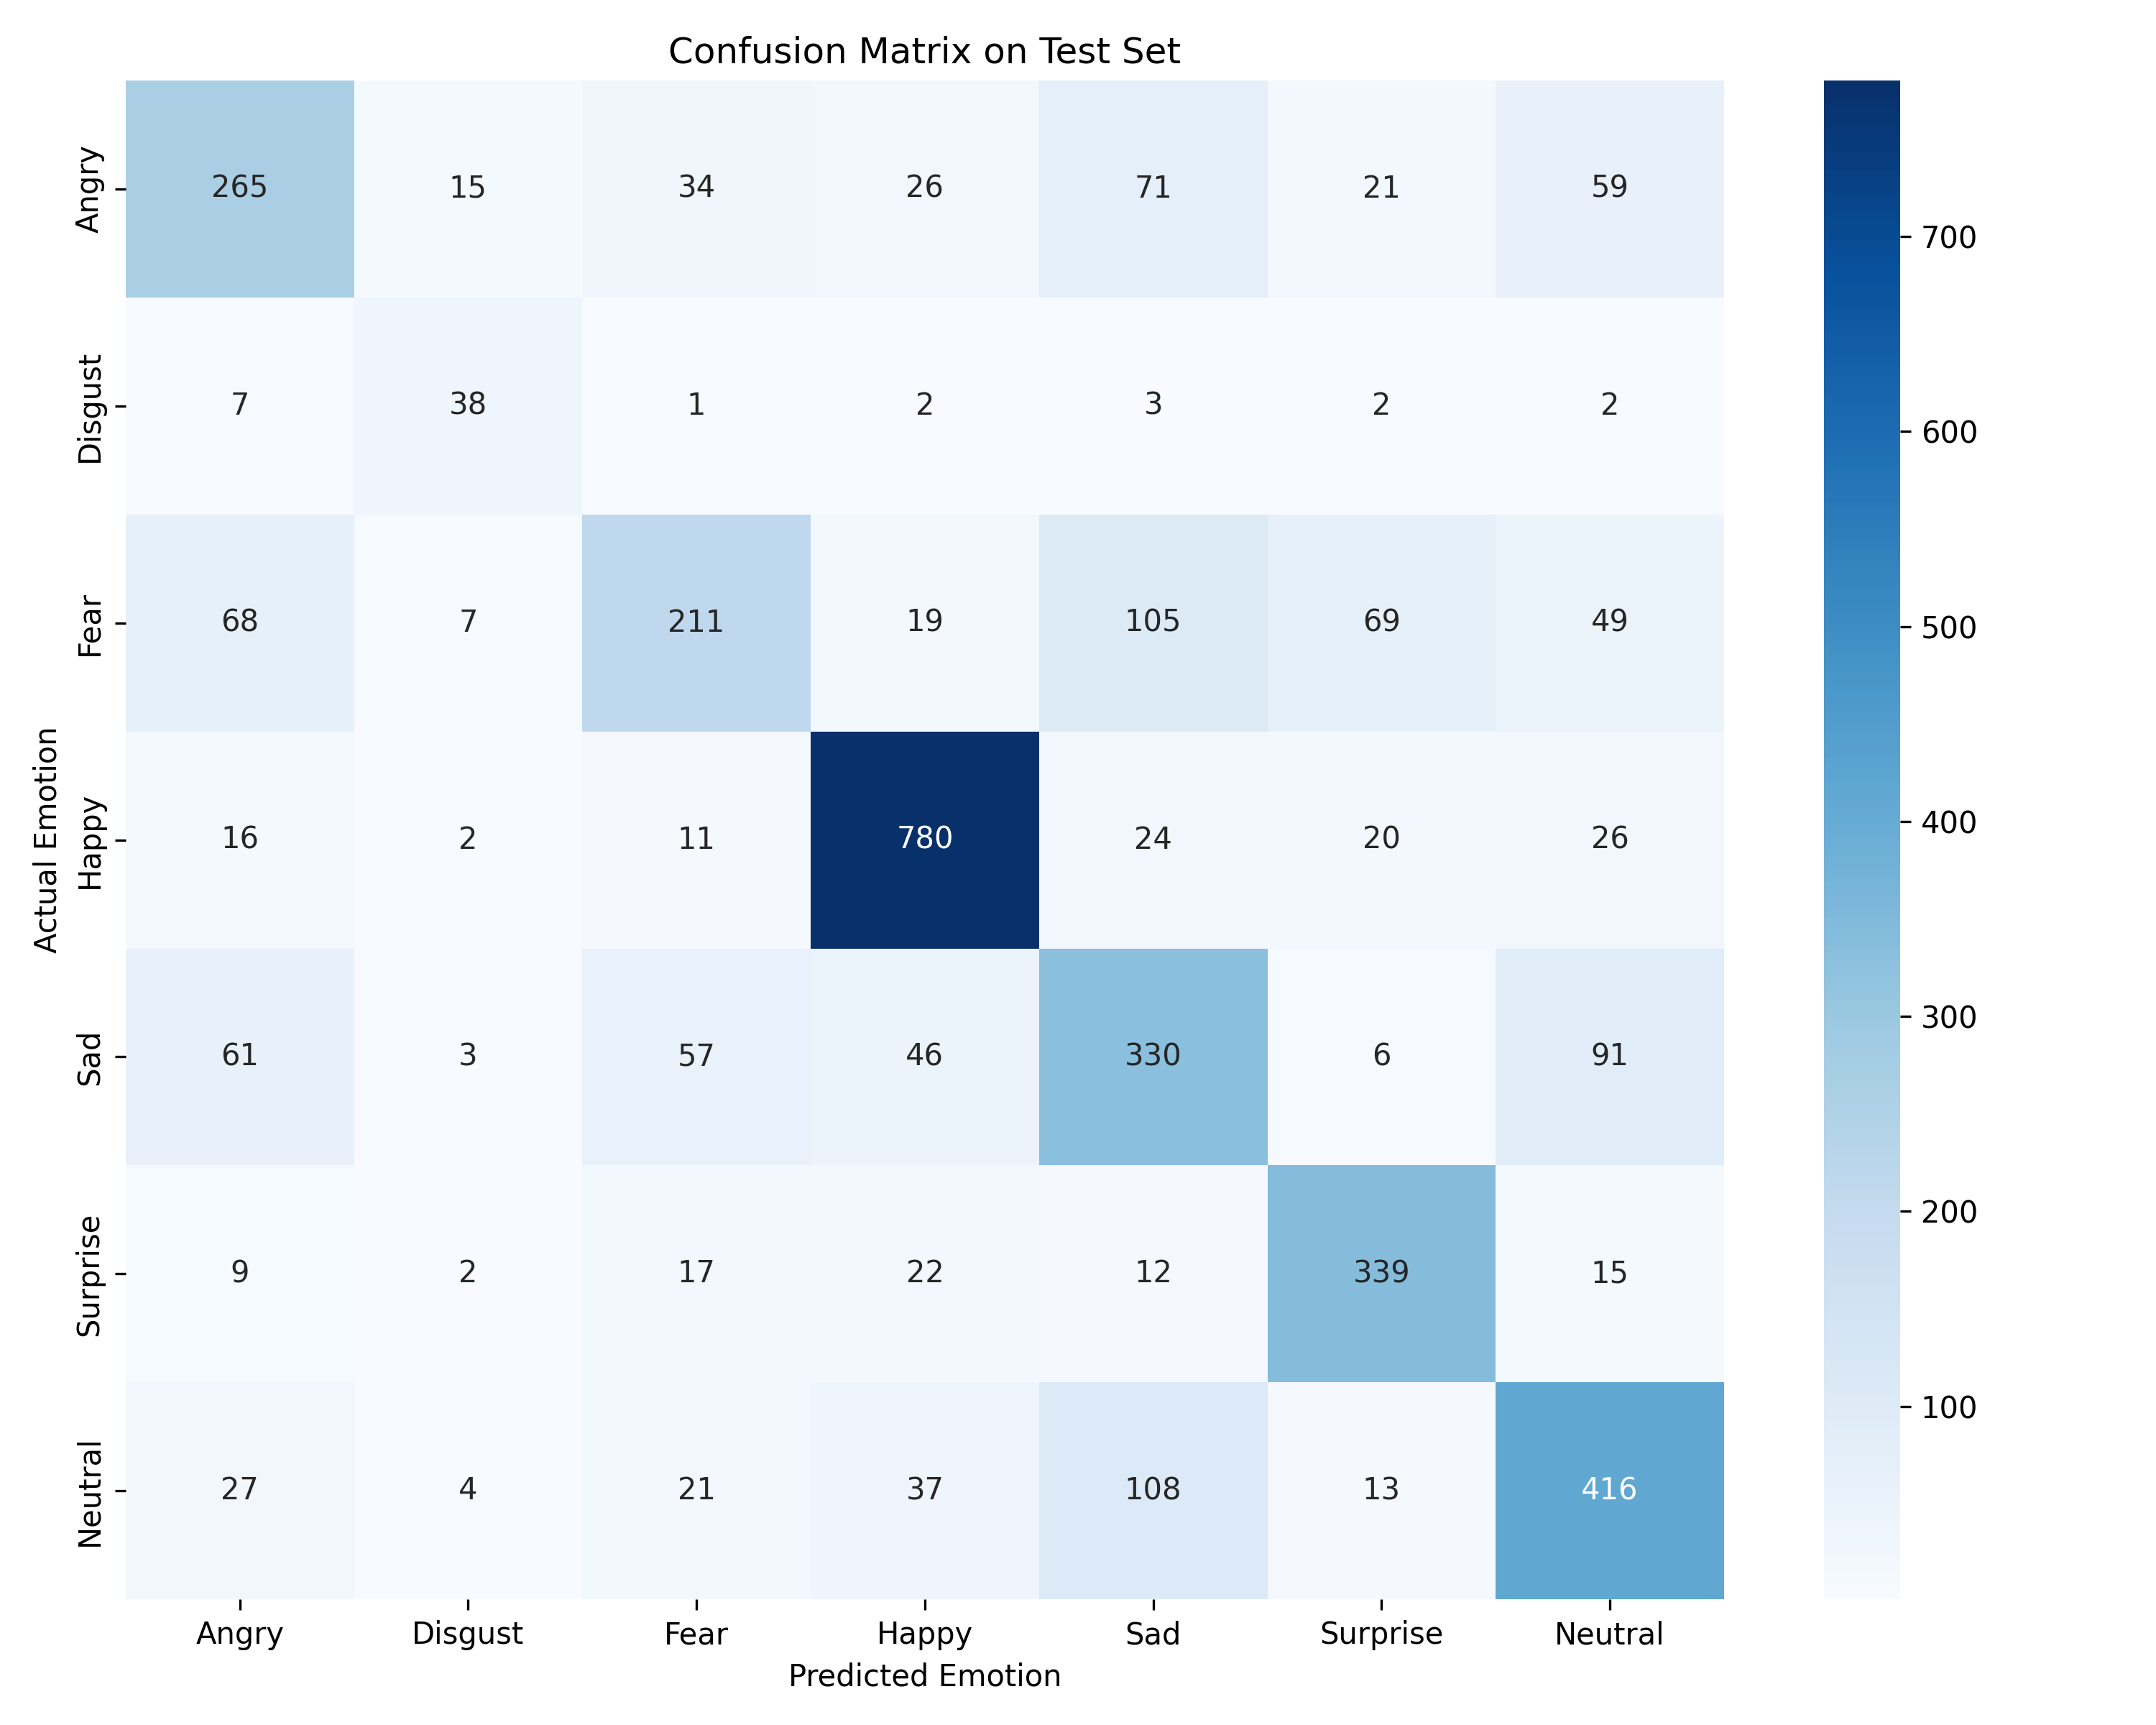
\includegraphics[width=0.85\textwidth]{images/confusion_matrix.png}
    \caption{ماتریس درهم‌ریختگی بهبودیافته پس از \lr{Fine-Tuning}}
    \label{fig:cm2}
\end{figure}

\subsubsection*{دستاوردها و تحلیل خطاهای باقیمانده:}
\begin{enumerate}
    \item \textbf{جهش در کلاس اقلیت:} بزرگترین دستاورد این روش، بهبود خیره‌کننده‌ی کلاس انزجار \lr{(Disgust)} است. در حالی که این کلاس تنها ۵۵ نمونه داشت، \lr{Recall} آن از \lr{2\%} در مدل قبلی به \lr{69\%} در این مدل جهش کرد که نشان می‌دهد لایه‌های آزادشده به خوبی توانسته‌اند ویژگی‌های خاص این احساس را یاد بگیرند.
    \item \textbf{تثبیت احساسات اصلی:} شادی با تشخیص \lr{780} نمونه و تعجب با \lr{339} نمونه، موفق‌ترین احساسات بوده‌اند. این دو احساس به دلیل تغییرات واضح در حالت دهان و چشم‌ها، راحت‌تر توسط شبکه‌های کانولوشنی استخراج می‌شوند.
    \item \textbf{تداخل بیولوژیکی:} بیشترین اشتباه شبکه، تشخیص احساس غم \lr{(Sad)} به جای خنثی \lr{(Neutral)} با ۱۰۸ خطا است. این تداخل از نظر بیولوژیکی و روان‌شناختی نیز کاملاً توجیه‌پذیر است، چرا که در بسیاری از چهره‌ها، حالت خنثی شباهت هندسی بسیار زیادی به چهره‌ی اندوهگینِ بدون واکنش دارد.
\end{enumerate}